%
%   Data Clarification
%       - Plots...
%   
\section{Data clarification}
\label{section:data_clarify}

\begin{figure}[H]
    \centering
    \begin{subfigure}[b]{0.49\textwidth}
        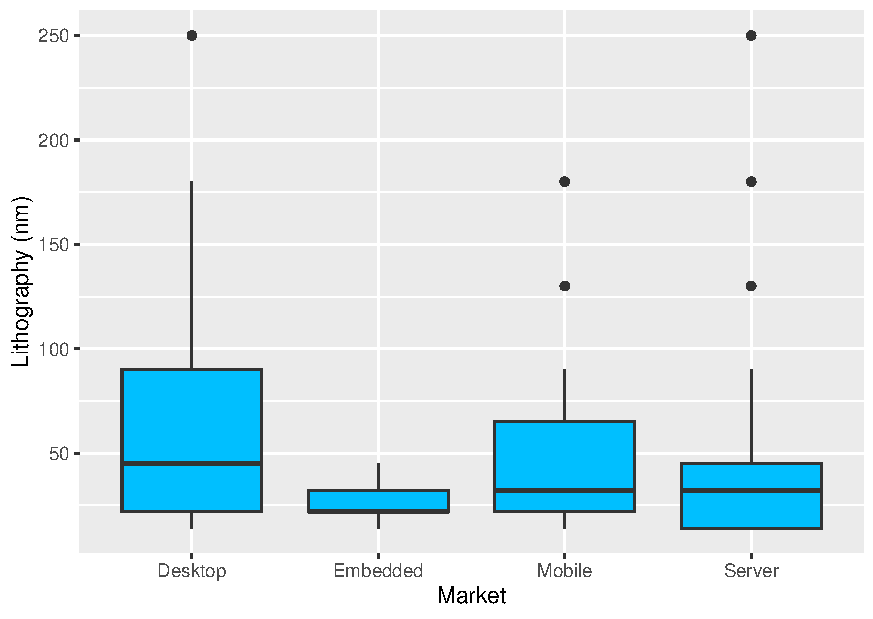
\includegraphics[width=\textwidth]{./graphics/box_litho.pdf}
        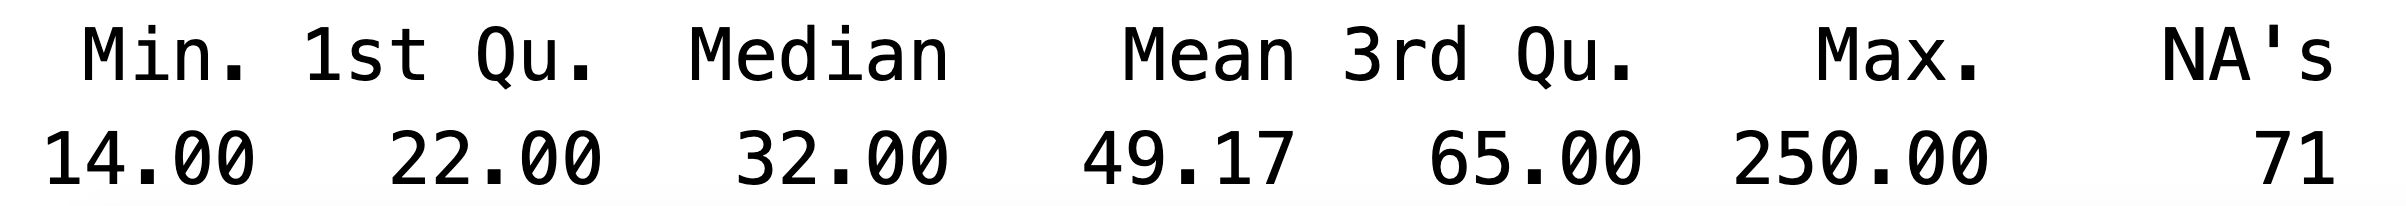
\includegraphics[width=\textwidth]{./graphics/sum_litho.png}
        \caption{Box plots and Summary of Lithography}
        \label{fig:box_litho}
    \end{subfigure}
    \hfill
    \begin{subfigure}[b]{0.49\textwidth}
        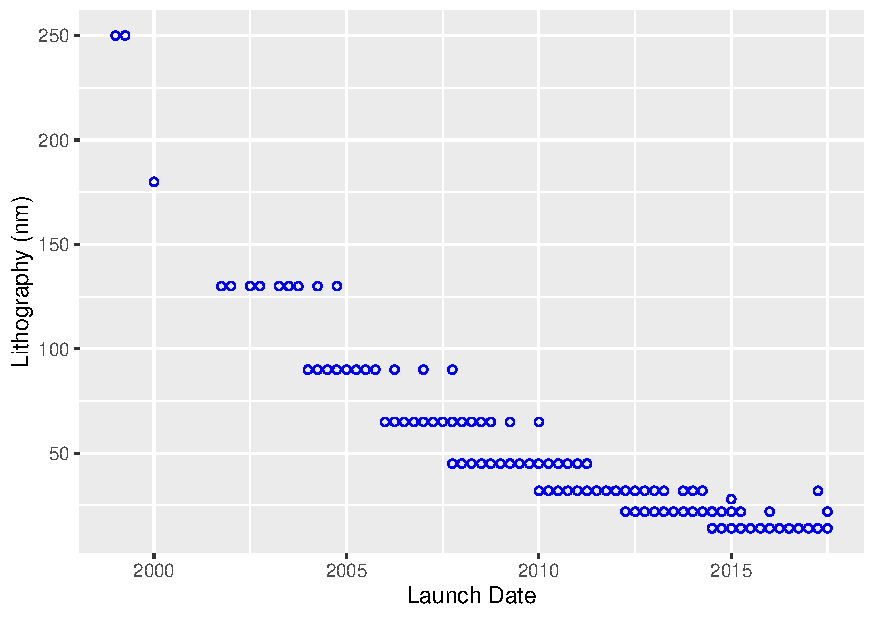
\includegraphics[width=\textwidth]{./graphics/scatter_litho.pdf}
        \caption{Plot of lithography over time.}
        \label{fig:scatter_litho}
    \end{subfigure}
    \caption{Lithography plots}
\end{figure}

\begin{code}{R}
ggplot(data, aes(x = market, y = litho)) +
    geom_boxplot(fill="deepskyblue") +
    labs(x = "Market", y = "Lithography (nm)")
  
summary(data$litho)

ggplot(data, aes(x = ldate, y = litho)) +
    geom_point(shape=1,color="blue") +
    labs(x = "Launch Date", y = "Lithography (nm)")
\end{code}

The scatter plot of \textit{Lithography} \textbf{[Figure \ref{fig:scatter_litho}]} 
shows that it is getting smaller over time, and is categorized into specific time intervals.
\textit{Lithography} spans the distribution over an interval of time  make it more powerful than \textit{Launch date}. In our
models, we always use \textit{Lithography} instead of \textit{Launch date}.









\begin{figure}[H]
    \centering
    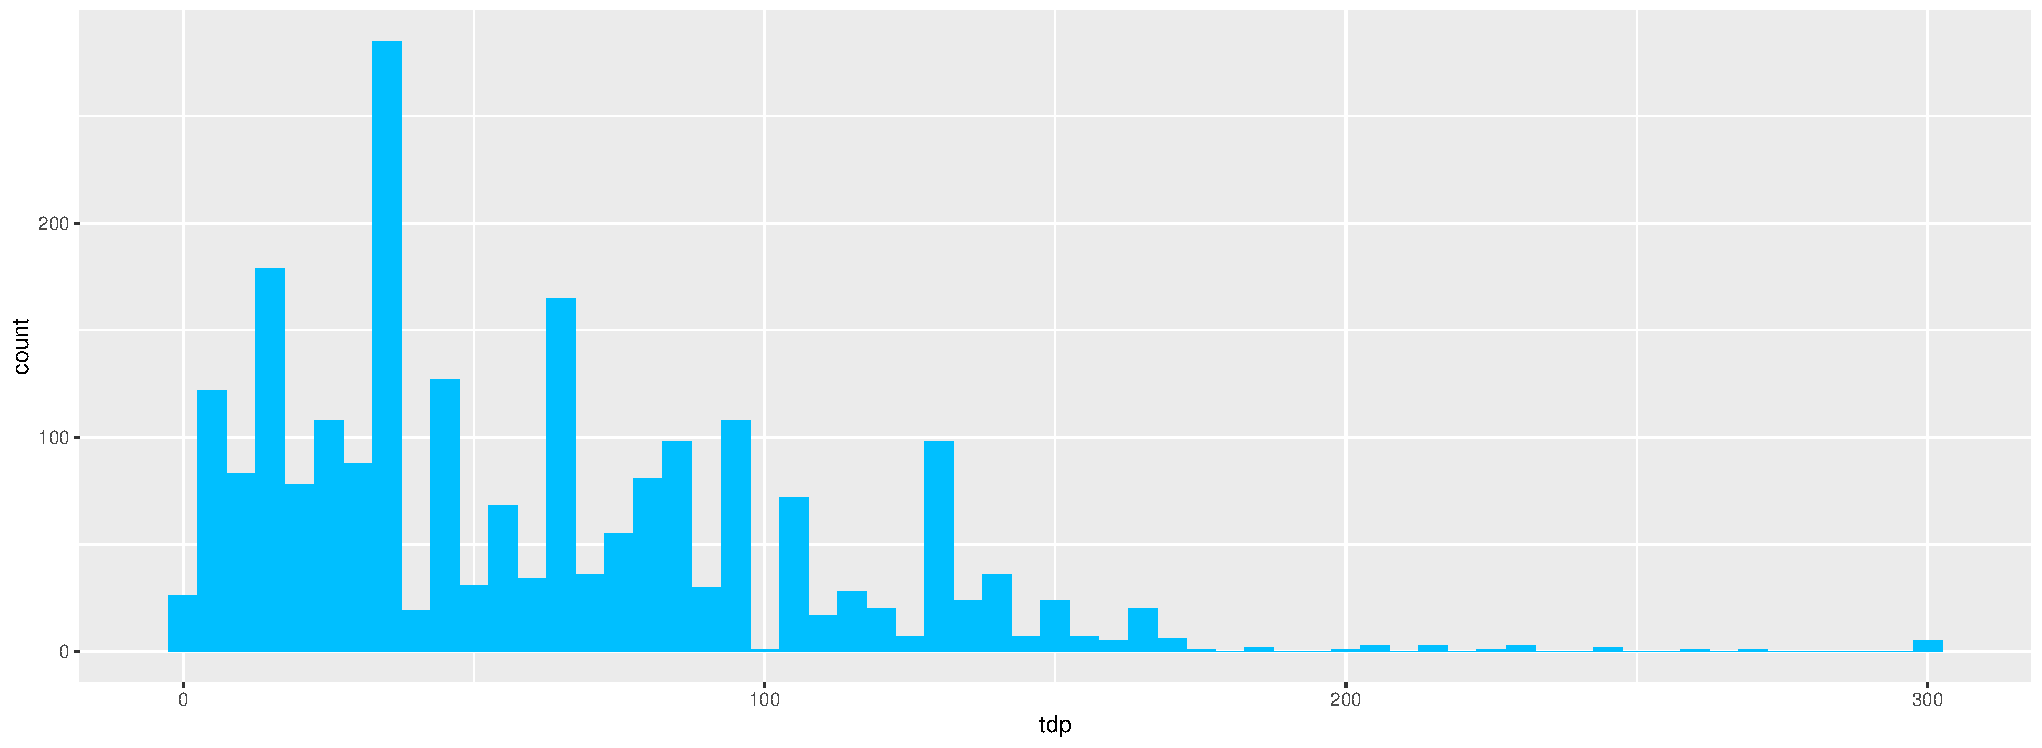
\includegraphics[width=0.75\textwidth]{./graphics/hist_tdp.pdf}
    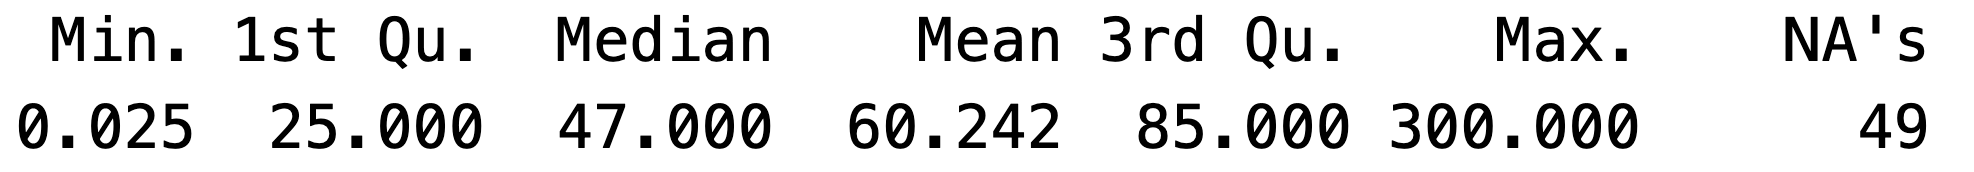
\includegraphics[width=0.75\textwidth]{./graphics/sum_tdp.png}
    \caption{Histogram and Summary of Thermal Design Power}
    \label{fig:hist_tdp}
\end{figure}

\begin{code}{R}
ggplot(data, aes(x = market,y = tdp)) +
    geom_boxplot(fill="deepskyblue") +
    labs(x = "Market", y = "Thermal deisgn power (W)")
  
  summary(data$tdp)
\end{code}

\textbf{[Figure \ref{fig:hist_tdp}]} The occurences of values $\ge 150$W are very rare, 
so they could be treated as outliners in further analysis.









\begin{figure}[H]
    \centering
    \begin{subfigure}[b]{0.45\textwidth}
        \centering
        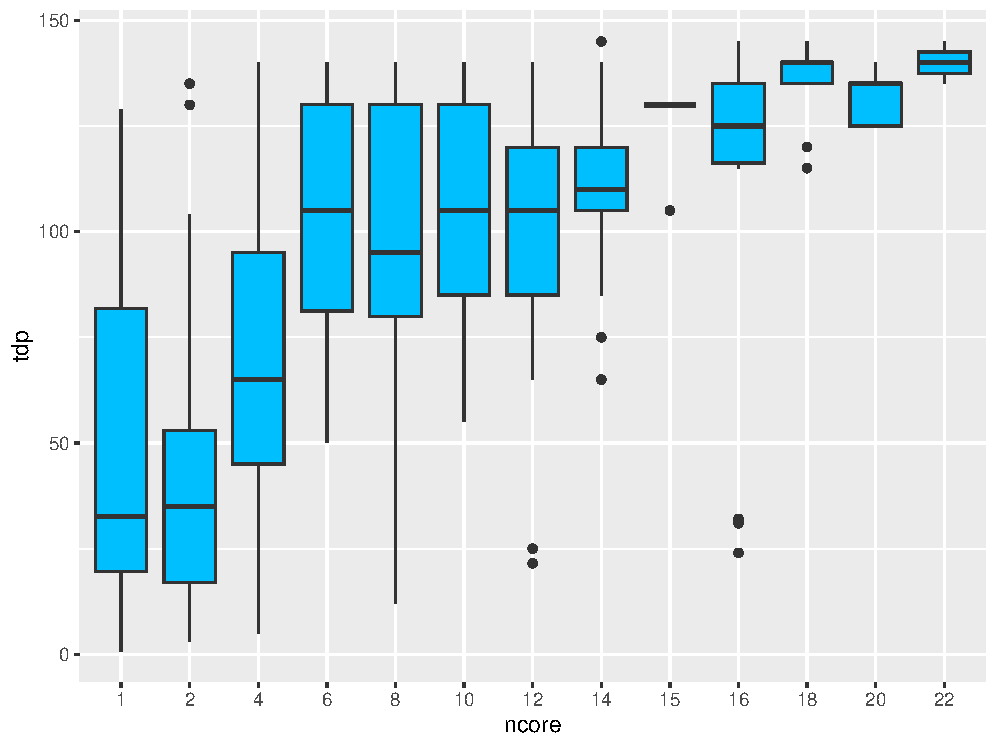
\includegraphics[width=\textwidth]{./graphics/box_tdp_ncore.pdf}
        \caption{Increasing trend of no. cores and TDP}
    \end{subfigure}
    \hfill
    \begin{subfigure}[b]{0.45\textwidth}
        \centering
        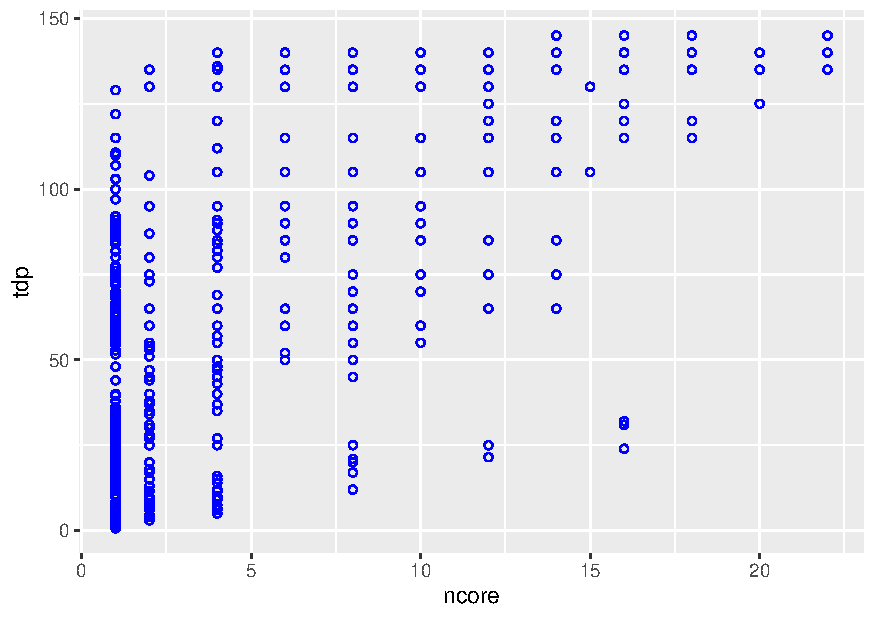
\includegraphics[width=\textwidth]{./graphics/scatter_tdp_ncore.pdf}
        \caption{Increasing trend of no. cores and TDP}
        \label{fig:tdp_analysis_ncore}
    \end{subfigure}
    \hfill
    \begin{subfigure}[b]{0.45\textwidth}
        \centering
        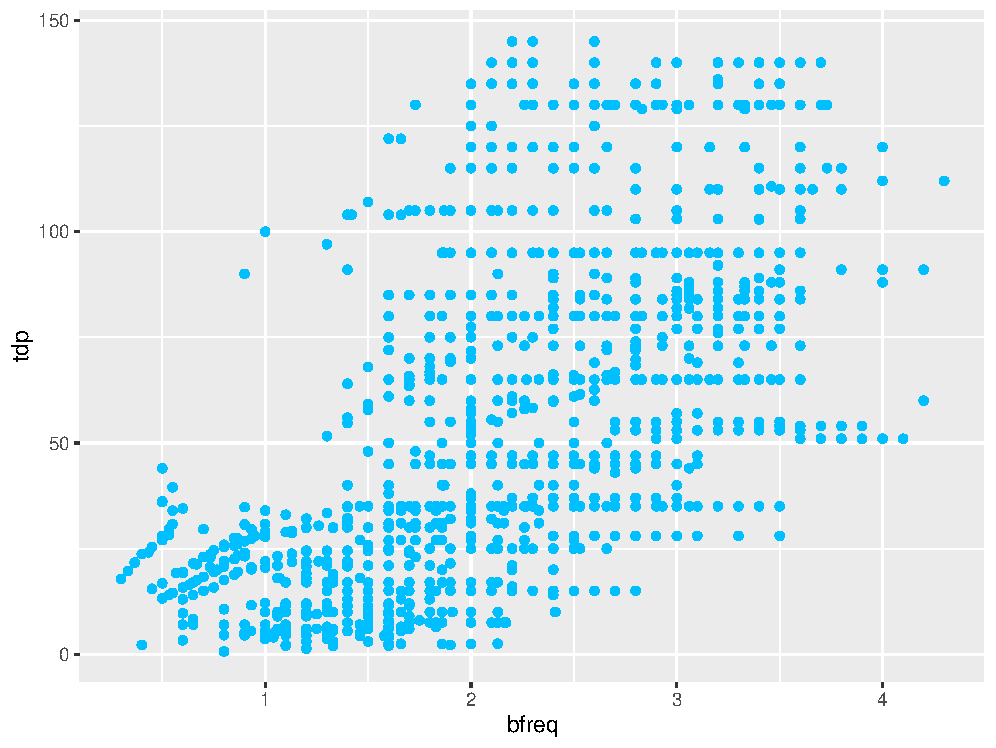
\includegraphics[width=\textwidth]{./graphics/scatter_tdp_bfreq.pdf}
        \caption{Increasing trend of Base frequency and TDP}
        \label{fig:tdp_analysis_bfreq}
    \end{subfigure}
    \hfill
    \begin{subfigure}[b]{0.45\textwidth}
        \centering
        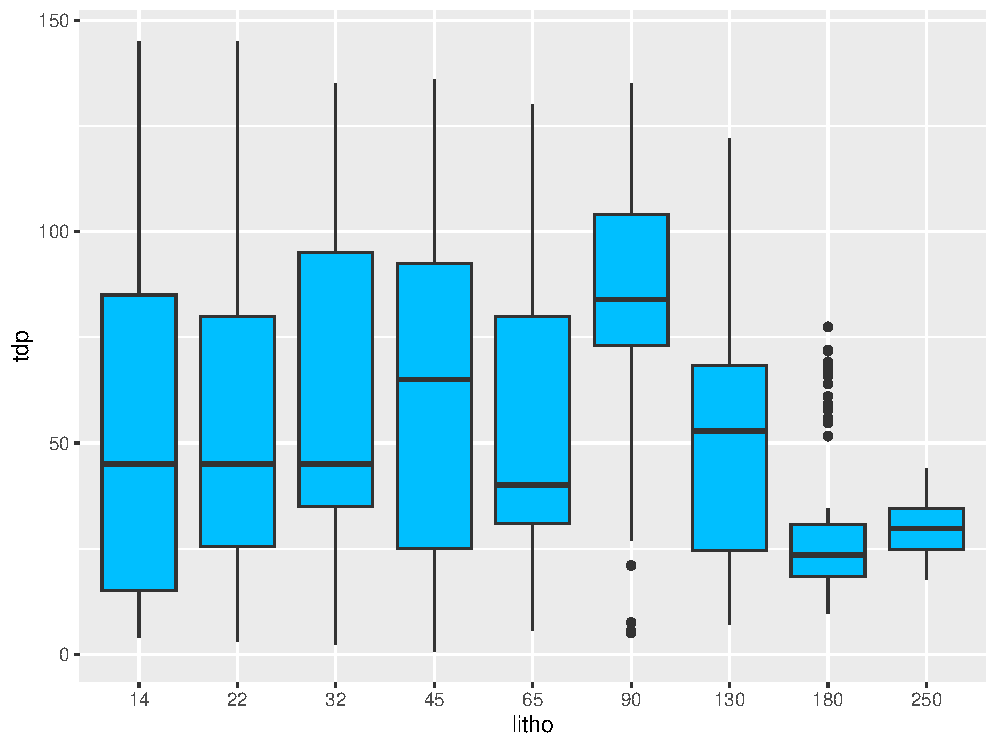
\includegraphics[width=\textwidth]{./graphics/box_tdp_litho.pdf}
        \caption{TDP within different Lithography}
        \label{fig:tdp_analysis_litho}
    \end{subfigure}
    \hfill
    \begin{subfigure}[b]{0.45\textwidth}
        \centering
        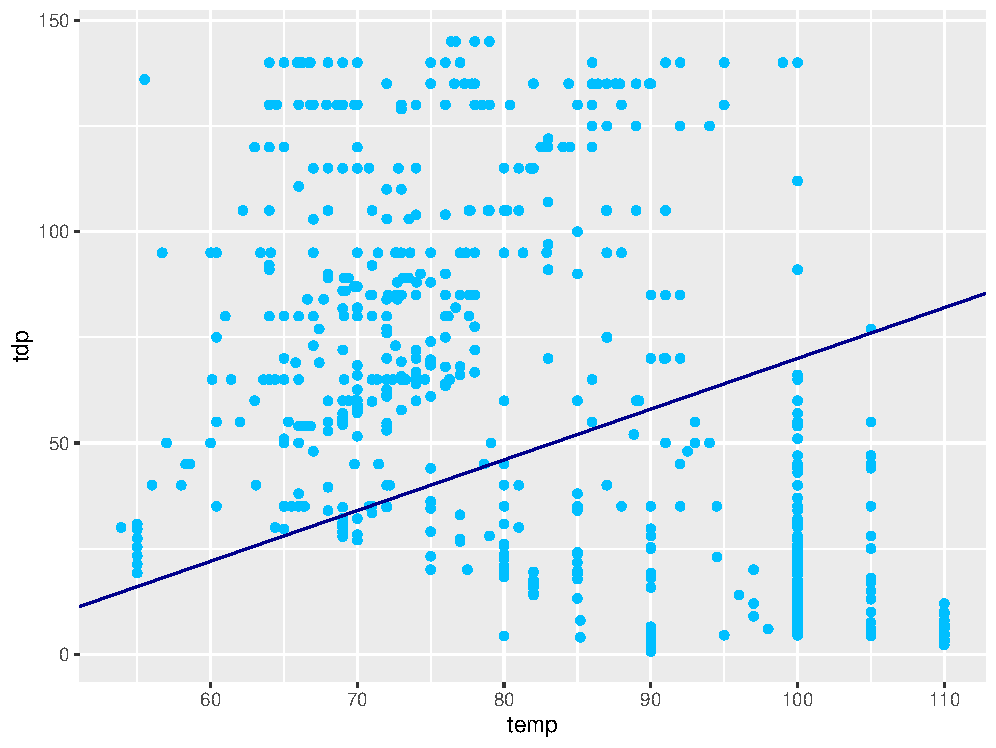
\includegraphics[width=\textwidth]{./graphics/scatter_tdp_temp.pdf}
        \caption{Different trends of TDP on different ranges of temperature}
        \label{fig:tdp_analysis_temp}
    \end{subfigure}
    \hfill
    \begin{subfigure}[b]{0.45\textwidth}
       \centering
       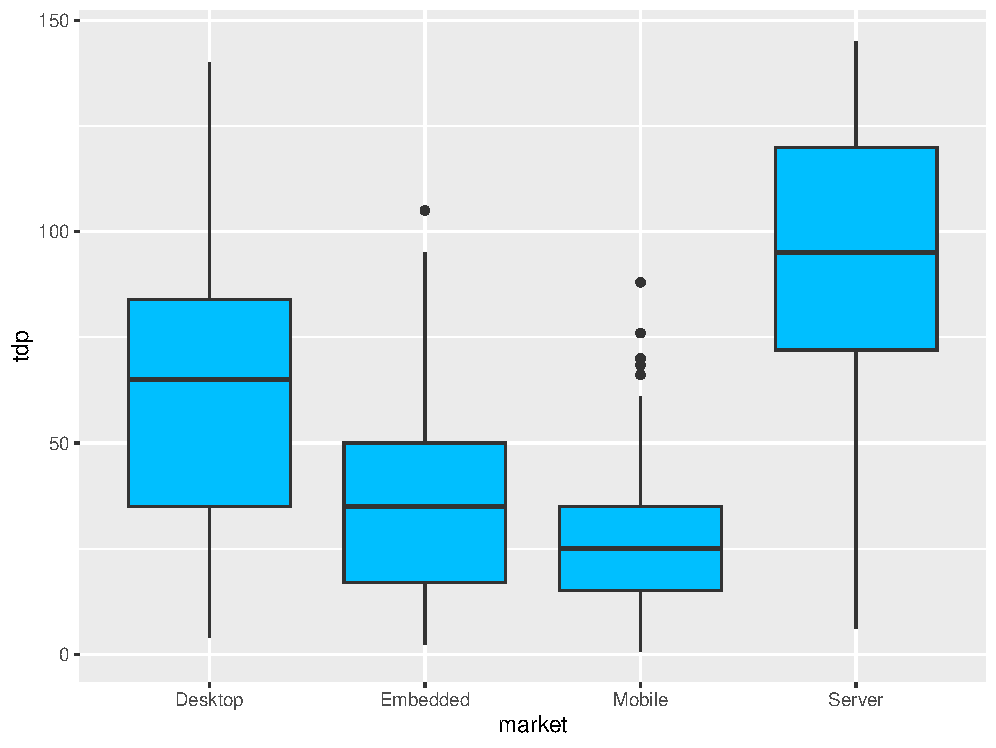
\includegraphics[width=\textwidth]{./graphics/box_tdp_market.pdf}
       \caption{Differences of TDP in different Markets}
       \label{fig:tdp_analysis_market}
    \end{subfigure}

    \caption{The relationship visualizations between TDP and other factors}
    \label{fig:tdp_analysis}
\end{figure}

From the above visualizations, we could make a few comments from these relationships, which motivates us to use certain Regression models:
\begin{itemize}
    \item \textbf{[Figure \ref{fig:tdp_analysis_ncore}]} \verb|tdp ~ ncore| : As \verb|ncore| increases, \verb|TDP| also increases. This motivates us to use 
    a Linear regression model. However, we also observe that, there are distinctive "clusters" on different ranges. Maybe a decision-based model, like Random Forrest,
    is better.
    
    \item \textbf{[Figure \ref{fig:tdp_analysis_bfreq}]} \verb|tdp ~ bfreq| : The data for this relationship is quite variant. However, the dominant trend is still linearly increasing,
    using Linear regression can be reliable.
    
    \item \textbf{[Figure \ref{fig:tdp_analysis_litho}]} \verb|tdp ~ litho| : There is no clear upward and downward trend. Instead, \verb|TDP| is converging and gets more and more stable over time. 
    
    \item \textbf{[Figure \ref{fig:tdp_analysis_temp}, \ref{fig:tdp_analysis_market}]} \verb|tdp ~ temp| and \verb|tdp ~ market| : There are two different trends happening: 
    above the reference line is increasing trend, while below is decreasing trend. In fact, we have a feeling that these two trends come from 
    different market segments \verb|type=(Desktop + Server) or (Mobile + Embedded)|, so we would plot them out to verify:

        \begin{code}{R}
data$type <- ifelse(data$market == 'Server' | data$market == 'Desktop', "Computers", "Devices")
data$type <- as.factor(data$type)

ggplot(data, aes(x = type, y = tdp)) +
geom_boxplot(fill="deepskyblue")
            
ggplot(data, aes(x = temp, y = tdp)) +
geom_point(color="deepskyblue", ) +
facet_wrap(~data$type)
        \end{code}

        \begin{figure}[H]
            \centering
            \begin{subfigure}[]{0.4\textwidth}
                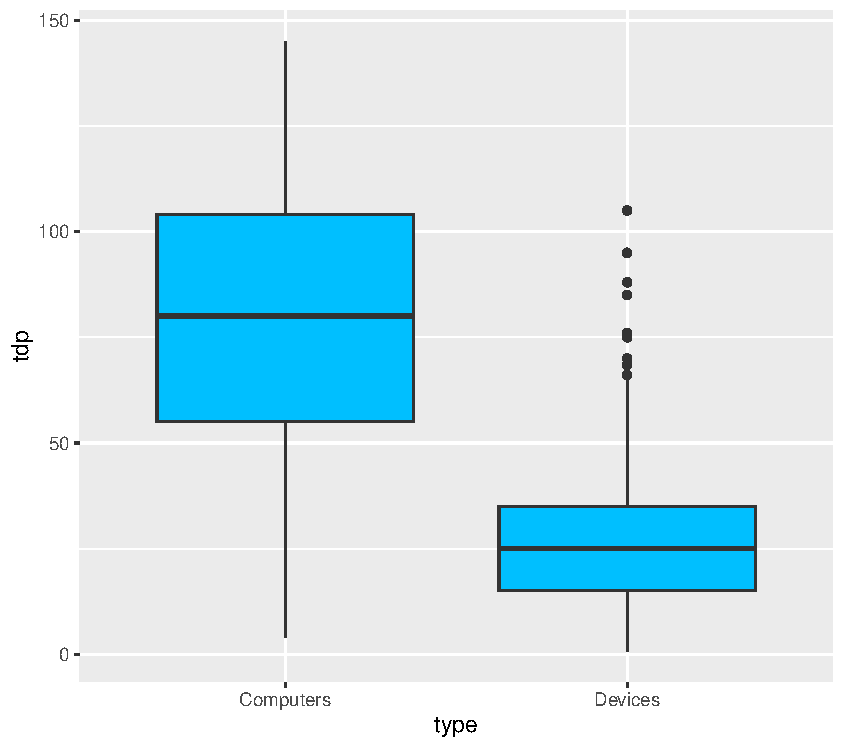
\includegraphics[width=\textwidth]{./graphics/box_tdp_type.pdf}
                \caption{TDP between Types.}
            \end{subfigure}
            \begin{subfigure}[]{0.4\textwidth}
                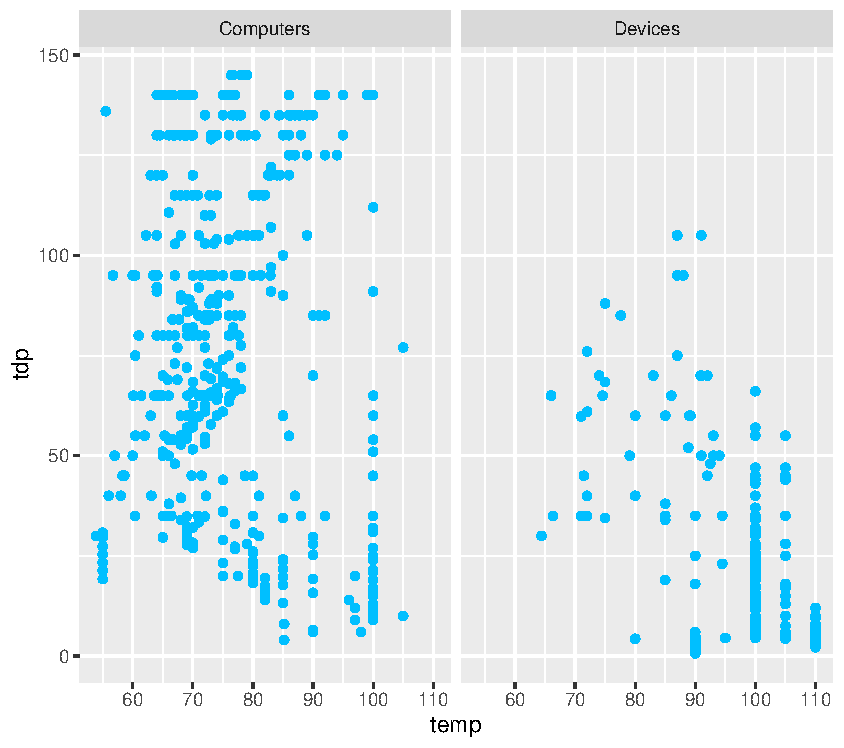
\includegraphics[width=\textwidth]{./graphics/scatter_type_tdp_temp.pdf}
                \caption{TDP in different Market segmentation}
            \end{subfigure}
        \end{figure}

    Turns out, different trends belongs to different Market segments (\verb|type|). This could be helpful for us to classify the \verb|TDP| into different markets
    using Logistic regression.
\end{itemize}